%%%%%%%%%%%%%%%%%%%%%%%%%%%%%%%%%%%%%%%%%%%%%%%%%%%%%%%%%%%%%%
% CHAPTER 6
%%%%%%%%%%%%%%%%%%%%%%%%%%%%%%%%%%%%%%%%%%%%%%%%%%%%%%%%%%%%%%

\chapter{System Implementation}
\label{chap:system_implementation}
\markboth{Chapter \thechapter: System Implementation}{}

%%%%%%%%%%%%%%%%%%%%%%%%%%%%%%%%%%%%%%%%%%%%%%%%%%%%%%%%%%%%%%
\section{Introduction}

This chapter describes the implementation of the proposed
\textbf{DocSaarthi: AI Legal \& Financial Document Assistant}.
The system is implemented as a bilingual document-intelligence
prototype that processes legal and financial PDF documents and
provides structured information to the user.

The implementation includes PDF upload and validation, text
extraction, language detection, legal/financial document
classification, key information extraction, document summarization,
bilingual retrieval, English--Hindi translation, and context-based
question answering. The system also provides page-level evidence so
that users can verify the generated information against the original
document.

The implementation was developed as a local prototype using
JavaScript and Node.js, with a 400-record Hindi intent dataset for
question-intent routing. Translation is provided through the Sarvam
translation API, while OpenAI-based answer generation is available as
an optional enhancement. The implementation focuses on maintaining the
uploaded document as the authoritative source of information.

%%%%%%%%%%%%%%%%%%%%%%%%%%%%%%%%%%%%%%%%%%%%%%%%%%%%%%%%%%%%%%
\section{Implementation Environment}

The DocSaarthi prototype was implemented using a web-based
client-server architecture. The backend handles document processing,
text extraction, classification, retrieval, translation, and answer
generation, while the frontend provides the user interface for
document upload and interaction.

\subsection{Hardware Environment}

The following hardware configuration is suitable for implementing and
testing the prototype.

\begin{table}[H]
\centering
\caption{Hardware Environment}
\begin{tabular}{|p{5cm}|p{8cm}|}
\hline
\textbf{Component} & \textbf{Configuration} \\
\hline
Processor & Intel Core i5 or equivalent processor \\
\hline
RAM & 8 GB minimum; 16 GB recommended \\
\hline
Storage & At least 10 GB free storage \\
\hline
GPU & Not mandatory for the implemented prototype \\
\hline
Internet Connectivity & Required for external translation services and optional AI services \\
\hline
\end{tabular}
\end{table}

\subsection{Software Environment}

\begin{table}[H]
\centering
\caption{Software Environment}
\begin{tabular}{|p{5cm}|p{8cm}|}
\hline
\textbf{Software / Technology} & \textbf{Purpose} \\
\hline
Operating System & Windows 10/11 or equivalent \\
\hline
Programming Language & JavaScript \\
\hline
Runtime Environment & Node.js 20 or later \\
\hline
Frontend & HTML, CSS and JavaScript \\
\hline
Backend & Node.js based server application \\
\hline
PDF Processing & pdfjs-dist \\
\hline
Translation & Sarvam Translation API \\
\hline
Optional AI Service & OpenAI API \\
\hline
Dataset Format & CSV \\
\hline
Version Control & Git / GitHub \\
\hline
\end{tabular}
\end{table}

%%%%%%%%%%%%%%%%%%%%%%%%%%%%%%%%%%%%%%%%%%%%%%%%%%%%%%%%%%%%%%
\section{Dataset Implementation}

The implemented system uses a labelled dataset containing
\textbf{400 records} for intent classification. The dataset is used
primarily for understanding and routing user queries rather than as
the evidence source for answering questions about uploaded documents.

The dataset contains Hindi-language intent examples representing
different types of user queries related to legal and financial
documents. The dataset is stored in CSV format and is loaded by the
application during execution.

The document itself remains the primary source of truth. Therefore,
information from the intent dataset is not directly used as evidence
for answering document-related questions.

\subsection{Dataset Loading}

The dataset is loaded by the application from the configured CSV
file. During initialization, the system checks whether the dataset is
available and loads the records required for intent identification.

The implementation also provides a dataset inspection utility to
check the number and distribution of records before execution.

\subsection{Dataset Usage}

The dataset is used for the following purposes:

\begin{itemize}
    \item Identifying the probable intent of a user's question.
    \item Routing questions to the appropriate document-processing
    logic.
    \item Supporting bilingual question handling.
    \item Improving the interaction between the user and the document
    assistant.
\end{itemize}

The dataset is not treated as authoritative evidence for document
answers. This separation helps prevent unrelated training examples
from being incorrectly presented as information extracted from the
uploaded document.

%%%%%%%%%%%%%%%%%%%%%%%%%%%%%%%%%%%%%%%%%%%%%%%%%%%%%%%%%%%%%%
\section{Preprocessing Implementation}

The preprocessing stage converts the extracted PDF content into a
clean and searchable textual representation. Since legal and financial
documents contain important numbers, dates, percentages, names, and
special symbols, preprocessing is performed carefully to avoid
removing meaningful information.

The implemented preprocessing pipeline consists of PDF text
extraction, Unicode normalization, line-break handling, duplicate
removal, text cleaning, tokenization, and document chunking.

\subsection{PDF Text Extraction}

The uploaded PDF is processed page by page using the
\texttt{pdfjs-dist} library. The extracted text is associated with its
corresponding page number.

This page-level representation is important because the system uses
the original page as evidence when displaying answers to the user.

\subsection{Text Cleaning}

The extracted text is cleaned before further processing. The
implementation handles unnecessary line breaks, repeated whitespace,
and common formatting inconsistencies while preserving important
information such as:

\begin{itemize}
    \item Names
    \item Dates
    \item Monetary values
    \item Percentages
    \item Legal clauses
    \item Financial terms
    \item Document identifiers
\end{itemize}

\subsection{Unicode Normalization}

Unicode normalization is applied to ensure that visually similar
characters are represented consistently. This is particularly
important for Hindi text because Devanagari characters may contain
combining marks.

The preprocessing stage therefore preserves Devanagari characters
instead of applying aggressive character removal.

\subsection{Document Chunking}

Long documents are divided into smaller text chunks before retrieval
and translation. Chunking allows the system to search relevant
sections efficiently and prevents excessively long text from being
sent to external translation or AI services.

Each chunk retains its relationship with the original document page,
allowing the final answer to provide page-level evidence.

%%%%%%%%%%%%%%%%%%%%%%%%%%%%%%%%%%%%%%%%%%%%%%%%%%%%%%%%%%%%%%
\section{Feature Representation Implementation}

The implemented prototype uses a combination of lexical and
structured textual representations rather than training a new
transformer model from scratch.

The extracted document text is represented using normalized tokens
and searchable text chunks. Token sets are used internally for
matching user queries with relevant document sections.

\subsection{Lexical Representation}

Important terms from the document and user query are normalized and
represented as token sets. These representations are used for
retrieval and matching.

For example, a query containing terms such as ``loan'', ``interest'',
``penalty'', or ``payment'' can be matched against relevant portions
of the uploaded financial document.

\subsection{Bilingual Representation}

The system supports English and Hindi interaction. A Hindi question
can be processed against English document content by using the
translation and retrieval layer.

Similarly, English queries can retrieve information from content that
has been translated or represented in Hindi.

This provides cross-language retrieval without modifying the
authoritative original document.

\subsection{Structured Information Representation}

In addition to textual chunks, the system maintains structured
information extracted from the document, including:

\begin{itemize}
    \item Dates
    \item Monetary values
    \item Percentages
    \item Important clauses
    \item Potential risk signals
    \item Document classification
    \item Page references
\end{itemize}

These representations help the system provide more useful and
verifiable responses.

%%%%%%%%%%%%%%%%%%%%%%%%%%%%%%%%%%%%%%%%%%%%%%%%%%%%%%%%%%%%%%
\section{Model Implementation}

The implementation uses a multi-stage approach rather than a single
machine learning model.

\subsection{Document Classification}

The uploaded document is classified as either \textbf{Legal} or
\textbf{Financial}. The current prototype uses document-content
analysis and heuristic/lexical signals to determine the most probable
category.

The system also provides a confidence value along with the predicted
category.

\subsection{Language Detection}

The system detects whether the uploaded document contains English,
Hindi, or mixed-language content. This information is used to
determine the appropriate processing and translation flow.

\subsection{Key Information Extraction}

The implementation identifies important information from the
document, including dates, monetary amounts, percentages, and
potentially important clauses.

Regular expressions and domain-specific lexical patterns are used for
extracting structured values.

\subsection{Question Answering}

The question-answering component follows a source-grounded approach.
The user submits a question in English or Hindi. The system searches
the indexed document chunks and retrieves the most relevant evidence.

The answer is generated only from the retrieved document content.
When sufficient evidence cannot be found, the system is designed to
return a ``not found'' response rather than inventing information.

\subsection{Translation}

English--Hindi translation is implemented using the Sarvam translation
API. Translation is treated as a separate convenience layer and does
not replace the original document.

The system supports:

\begin{itemize}
    \item English-to-Hindi translation.
    \item Hindi-to-English translation where required.
    \item Hindi summaries.
    \item Bilingual question and answer interaction.
\end{itemize}

The implementation also includes text chunking and error handling for
long translation requests.

\subsection{Optional AI Answer Generation}

OpenAI-based answer generation is implemented as an optional
enhancement. It can generate more natural responses from retrieved
document evidence.

The OpenAI component is disabled unless the required configuration and
API key are explicitly provided. A local fallback mechanism is
available when the external AI service is unavailable.

%%%%%%%%%%%%%%%%%%%%%%%%%%%%%%%%%%%%%%%%%%%%%%%%%%%%%%%%%%%%%%
\section{Training Configuration}

The current DocSaarthi prototype does not perform large-scale
transformer pretraining or fine-tuning. Instead, pretrained services
and rule-based/lexical processing are combined to create a practical
document-intelligence prototype.

The 400-record intent dataset is loaded during application execution
and used for intent routing. The document-processing pipeline operates
on the uploaded PDF at runtime.

\begin{table}[H]
\centering
\caption{Training and Processing Configuration}
\begin{tabular}{|p{5cm}|p{8cm}|}
\hline
\textbf{Parameter} & \textbf{Configuration} \\
\hline
Intent Dataset & 400 labelled records \\
\hline
Dataset Format & CSV \\
\hline
Document Processing & Runtime processing of uploaded PDFs \\
\hline
Classification & Lexical/heuristic document analysis \\
\hline
Translation Model & Sarvam hosted translation service \\
\hline
Answer Generation & Local grounded logic with optional OpenAI enhancement \\
\hline
Retrieval & Document chunk and token-based matching \\
\hline
Model Fine-tuning & Not performed in the current prototype \\
\hline
GPU Requirement & Not mandatory \\
\hline
\end{tabular}
\end{table}

This configuration was selected because the project focuses on
demonstrating an integrated multilingual document-intelligence
pipeline within the available project resources.

%%%%%%%%%%%%%%%%%%%%%%%%%%%%%%%%%%%%%%%%%%%%%%%%%%%%%%%%%%%%%%
\section{Implementation Challenges and Solutions}

During implementation, several challenges were identified due to the
complexity of legal and financial documents and the requirement for
bilingual interaction.

\begin{table}[H]
\centering
\caption{Implementation Challenges and Solutions}
\begin{tabular}{|p{5cm}|p{8cm}|}
\hline
\textbf{Challenge} & \textbf{Implemented Solution} \\
\hline
Long PDF documents & Documents are divided into smaller searchable chunks. \\
\hline
PDF line-break inconsistencies & Text normalization and line-break handling are applied. \\
\hline
Hindi Unicode handling & Unicode normalization preserves Devanagari characters and combining marks. \\
\hline
English--Hindi interaction & Cross-language retrieval and translation are implemented. \\
\hline
Large translation input & Translation requests are divided into manageable chunks. \\
\hline
Important numbers and dates & Monetary values, percentages, and dates are explicitly preserved and extracted. \\
\hline
Unsupported questions & The system returns a safe ``not found'' response when sufficient evidence is unavailable. \\
\hline
Hallucination risk & Answers are grounded in retrieved document evidence. \\
\hline
External API failure & Fallback mechanisms and error handling are implemented. \\
\hline
Document verification & Page-level citations are retained with retrieved evidence. \\
\hline
\end{tabular}
\end{table}

%%%%%%%%%%%%%%%%%%%%%%%%%%%%%%%%%%%%%%%%%%%%%%%%%%%%%%%%%%%%%%
\section{Implemented System Architecture}

The implemented architecture follows a modular document-processing
workflow. The major stages of the system are shown below.

% Temporary placeholder for the architecture figure.
% Replace this block with the actual figure once the image is available.
\begin{figure}[H]
    \centering
    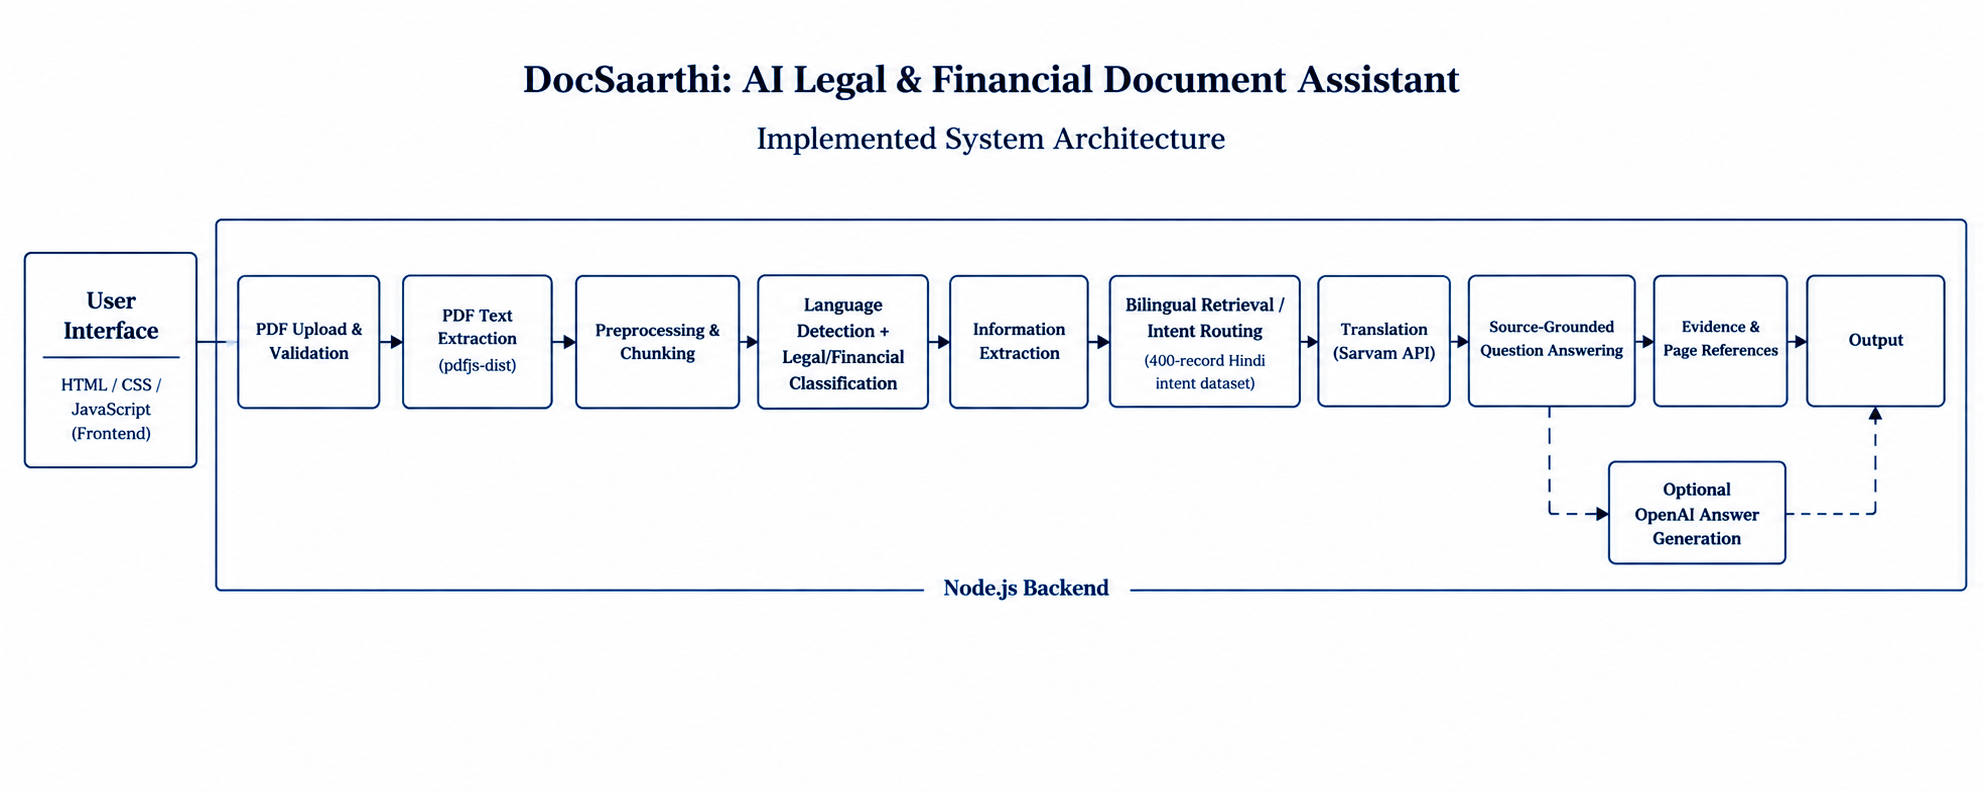
\includegraphics[width=\textwidth]{figures/implemented_system_architecture.png}
    \caption{Implemented System Architecture of DocSaarthi}
    \label{fig:implemented_architecture}
\end{figure}

The implemented system consists of the following major components:

\begin{enumerate}
    \item \textbf{User Interface:} Allows the user to upload documents,
    view results, and interact with the document assistant.

    \item \textbf{PDF Upload and Validation:} Validates the uploaded
    PDF and prepares it for processing.

    \item \textbf{PDF Text Extraction:} Extracts text from each page
    while preserving page information.

    \item \textbf{Preprocessing Module:} Performs text normalization,
    cleaning, and chunking.

    \item \textbf{Language Detection:} Identifies the language or
    language combination present in the document.

    \item \textbf{Document Classification:} Determines whether the
    document is primarily Legal or Financial.

    \item \textbf{Information Extraction:} Extracts dates, amounts,
    percentages, clauses, and potential risk signals.

    \item \textbf{Bilingual Retrieval:} Matches user questions with
    relevant document chunks in English or Hindi.

    \item \textbf{Translation Module:} Provides English--Hindi
    translation using the configured translation service.

    \item \textbf{Question Answering Module:} Generates answers based
    on retrieved document evidence.

    \item \textbf{Evidence and Citation Module:} Maintains page-level
    references so that users can verify the answer against the
    original document.

    \item \textbf{Output Module:} Displays classification, extracted
    information, summaries, translations, and question-answering
    results to the user.
\end{enumerate}

The implemented architecture follows a source-grounded design in
which the original uploaded document remains the authoritative source.
Translated content is maintained separately, and information from the
intent dataset is not used as evidence for document answers.

%%%%%%%%%%%%%%%%%%%%%%%%%%%%%%%%%%%%%%%%%%%%%%%%%%%%%%%%%%%%%%
\section*{Chapter Summary}

This chapter presented the implementation of the proposed
\textbf{DocSaarthi} system. The implementation environment, dataset
handling, preprocessing pipeline, feature representation, document
classification, information extraction, translation, and
question-answering components were described. The chapter also
discussed the processing configuration, implementation challenges and
their solutions, and the final implemented system architecture.

The implemented prototype integrates PDF processing, bilingual
interaction, document retrieval, structured information extraction,
translation, and source-grounded question answering into a single
workflow. The next chapter presents the experimental results and
evaluation of the implemented system.

%%%%%%%%%%%%%%%%%%%%%%%%%%%%%%%%%%%%%%%%%%%%%%%%%%%%%%%%%%%%%%